\documentclass[a4paper, 11pt]{article}
\usepackage{comment}
\usepackage{lipsum} 
\usepackage{fullpage} %cambiar margen
\usepackage[a4paper, total={7in, 10in}]{geometry}

\usepackage{amssymb,amsthm} 
\usepackage{amsmath}
\newtheorem{theorem}{Theorem}
\newtheorem{corollary}{Corollary}
\usepackage{graphicx}
\usepackage{tikz}
\usetikzlibrary{arrows}
\usepackage{verbatim}
%\usepackage[numbered]{mcode}
\usepackage{float}
\usepackage{tikz}
\usetikzlibrary{shapes,arrows}
\usetikzlibrary{arrows,calc,positioning}
\usepackage{mathpazo} %tipo de letra 
\usepackage[utf8]{inputenc} %codificación
\usepackage[T1]{fontenc} %digitación de tildes y ñ
\usepackage[spanish]{babel} %paquete de soporte español

\tikzset{
	block/.style = {draw, rectangle,
		minimum height=1cm,
		minimum width=1.5cm},
	input/.style = {coordinate,node distance=1cm},
	output/.style = {coordinate,node distance=4cm},
	arrow/.style={draw, -latex,node distance=2cm},
	pinstyle/.style = {pin edge={latex-, black,node distance=2cm}},
	sum/.style = {draw, circle, node distance=1cm},
}
\usepackage{xcolor}
\usepackage{mdframed}
\usepackage[shortlabels]{enumitem}
\usepackage{indentfirst}
\usepackage{hyperref}

\usepackage{listings}
\lstset{literate=
  {á}{{\'a}}1
  {é}{{\'e}}1
  {í}{{\'i}}1
  {ó}{{\'o}}1
  {ú}{{\'u}}1
  {Á}{{\'A}}1
  {É}{{\'E}}1
  {Í}{{\'I}}1
  {Ó}{{\'O}}1
  {Ú}{{\'U}}1
  {ñ}{{\~n}}1
  {ü}{{\"u}}1
  {Ü}{{\"U}}1
}

\lstdefinestyle{customc}{
  belowcaptionskip=1\baselineskip,
  breaklines=true,
  frame=L,
  xleftmargin=\parindent,
  language=Python,
  showstringspaces=false,
  basicstyle=\footnotesize\ttfamily,
  keywordstyle=\bfseries\color{green!40!black},
  commentstyle=\itshape\color{purple!40!black},
  identifierstyle=\color{blue},
  stringstyle=\color{orange},
}

\lstdefinestyle{customasm}{
  belowcaptionskip=1\baselineskip,
  frame=L,
  xleftmargin=\parindent,
  language=[x86masm]Assembler,
  basicstyle=\footnotesize\ttfamily,
  commentstyle=\itshape\color{purple!40!black},
}

\lstset{escapechar=@,style=customc}



\renewcommand{\thesubsection}{\thesection.\alph{subsection}}

\newenvironment{problem}[2][Ejercicio]
{ \begin{mdframed}[backgroundcolor= red!50] \textbf{#1 #2} \\}
	{  \end{mdframed}}

% Define solution environment
\newenvironment{solution}
{\textcolor{blue}{\textbf{\textit{Solución:\\\noindent}}}}


\renewcommand{\qed}{\quad\qedsymbol}

% \\	
\begin{document}
	\noindent
	%%%%%%%%%%%%%%%%%%%%%%%%%%%%%%%%%%%%
	
	\begin{minipage}[b][1.2cm][t]{0.8\textwidth}
		\large\textbf{César Isaí García Cornejo} \hfill \textbf{Tarea 7}  \\
		cesar.cornejo@cimat.mx \hfill \\
		\normalsize Computo Científico \hfill Semestre 3\\
	\end{minipage}
	
	\hspace{14.4cm}
	\begin{minipage}[b][0.03cm][t]{0.12\linewidth}
		
		\vspace{-2.2cm}
		%%%La Ruta dependerá de donde este alojado el main y la imagen
		
\includegraphics[scale=0.3]{Figures/EscudoCimat.png}
	\end{minipage}
	
	\noindent\rule{7in}{2.8pt}
	
	%%%%%%%%%%%%%%%%%%%%%
	%%%%%%%%%%%%%%%%%%%%%%%%%%%%%%%%%%%%%%%%%%%%%%%%%%%%%%%%%%%%%%%%%%%%%%%%%%%%%%%%%%%%%%%%%%%%%%%%%%%%%%%%%%%%%%%%%%%
	% Problem 1
	%%%%%%%%%%%%%%%%%%%%%%%%%%%%%%%%%%%%%%%%%%%%%%%%%%%%%%%%%%%%%%%%%%%%%%%%%%%%%%%%%%%%%%%%%%%%%%%%%%%%%%%%%%%%%%%%%%%%%%%%%%%%%%%%%%%%%%%%
	\setlength{\parskip}{\medskipamount}
	\setlength{\parindent}{0pt}
%/////////// Ejercicio 1 /////////////////
\textbf{Con el algoritmo de Metropolis-Hastings (MH), simular lo siguiente:}
\begin{problem}{1} 
  Sean $x_i \sim Ga(\alpha,\beta)$ $i =1,2,\cdots,n$. Simular datos $x_i$ con $\alpha = 3$ y $\beta = 100$ considerando los casos $n=4$ y 30.
  
  Con $\alpha \sim U(1,4)$, $\beta \sim exp(1)$ distribuciones a priori, se tiene la posterior 
  \begin{align*}
    f(\alpha, \beta|\bar{x} ) \propto \frac{\beta^{n\alpha}}{\Gamma(\alpha)}^{n }  r_1^{\alpha-1}e^{-\beta(r_2 + 1)} \mathbb{1}_{1 \leq \alpha \leq 4} \mathbb{1}_{b>1}
  \end{align*}
  con $r_2 = \sum_{i=1}^{n } x_i$ y $r_1 = \prod_{i =1}^{n }x_i$.
  En ambos casos, grafica los contornos para visualizar dónde está concentrada la posterior.
  Utilizar la propuesta
  \begin{align*}
    q \left(\binom{\alpha_p }{\beta_p }| \binom{\alpha}{\beta}\right) = \binom{\alpha}{\beta} + \binom{\varepsilon_1}{\varepsilon_2}
  \end{align*}
  donde
  \begin{align*}
    \binom{\varepsilon_1}{\varepsilon_2} \sim N \left(\binom{0}{0}, \begin{pmatrix}
      \sigma_1^2 &0 \\ 
      0 & \sigma_2^2 
      \end{pmatrix} \right)
  \end{align*}

\end{problem}

\begin{solution} 
  Se implementa el algoritmo de Metropolis- Hastings con caminatas aleatorias para la posterior mostrada en el enunciado para cada caso, es decir, $n=4$ y $n = 30$

  Se procede definiendo una función que calcule la distribución posterior según ciertos valores de $\alpha,\beta$. Como es una función bivariada, y con objetivo de visualizar la distribución posterior, es que se grafican las curvas de nivel. Notemos que el soporte está en $1 \leq \alpha \leq 4$ y $\beta > 0$. Tenemos las siguientes gráficas
  \begin{figure}[H] 
      \centering 
      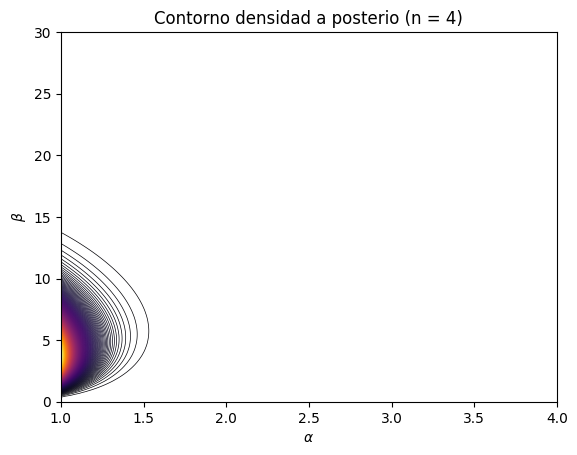
\includegraphics[width = 12 cm ]{Figures/contorno1.png} 
      \caption{Grafica de contornos para $n = 4$}
      \label{Fig. 1.01}
  \end{figure} 
  \begin{figure}[H] 
      \centering 
      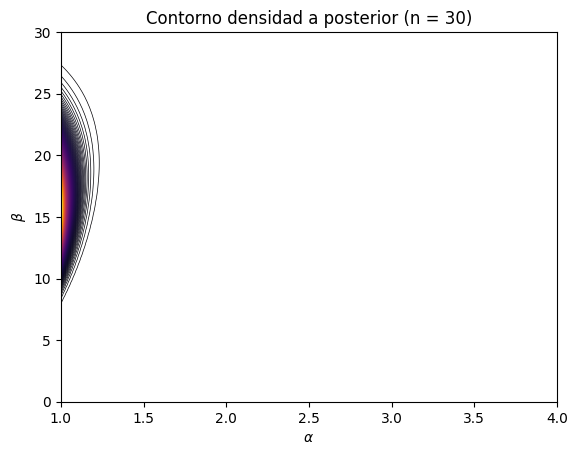
\includegraphics[width = 12 cm ]{Figures/contorno2.png} 
      \caption{Grafica de contornos para $n = 30$}
      \label{Fig. 1.02}
  \end{figure} 
  Notemos que tenemos una concentración para $\alpha $ pegados al extremos izquierdo del soporte, mientras que para $\beta$ se aglomeran por 5 o 15 dependiendo de $n$.

  Aplicando el método de Metropolis-Hastings con caminata aleatoria y punto inicial en $\alpha = 3,\beta = 40$ y propuesta como es indicada en el enunciado
  \begin{align*}
    \varepsilon_1 \sim N(0, \sigma_1^2) \:\:\:\:\:\: \varepsilon_2 \sim N(0,\sigma_2^2)
  \end{align*}
  con $\sigma_1 =$ 0.05 y $\sigma_2^2$ = 0.5
  
  Como la propuesta es simétrica, la probabilidad de transición es solamente el mínimo entre 1 y el cociente de la densidad a posteriori $f(\alpha_p,\beta_p|x) / f(\alpha,\beta|x)$ con $\alpha_p, \beta_p$ el siguiente valor propuesto. De esta forma, la cadena seguirá una caminata aleatoria en el plano como se puede ver en la siguiente figura
\begin{figure}[H] 
    \centering 
    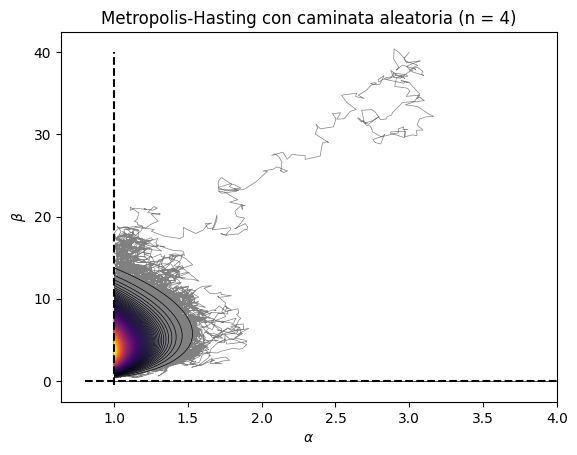
\includegraphics[width = 14 cm]{Figures/MHRW1.png} 
    \caption{Metropolis-Hastings con caminata aleatoria para la distribución a posteriori con $n = 4$  donde la distribución propuesta es una normal bivariada.}
    \label{Fig. 1.03 }
\end{figure} 
\begin{figure}[H] 
    \centering 
    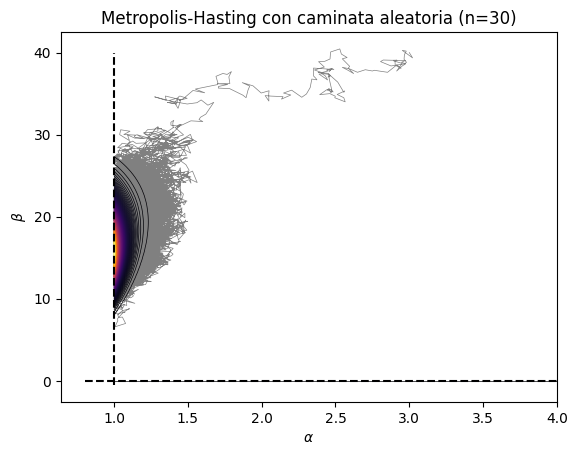
\includegraphics[width = 14cm]{Figures/MHRW2.png} 
    \caption{Metropolis-Hastings con caminata aleatoria para la distribución a posteriori con $n = 30$ donde la distribución propuesta es una normal bivariada.}
    \label{Fig. 1.04}
\end{figure} 

Posteriormente, se nos pide observar la evolución de la cadena de Markov
\begin{figure}[H] 
    \centering 
    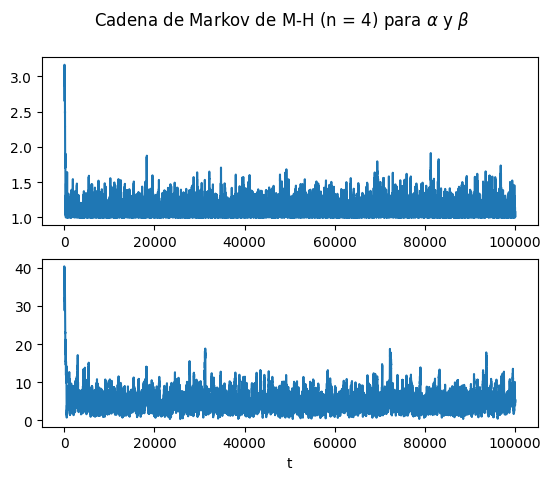
\includegraphics[width = 12 cm ]{Figures/cadenaMarkov1.png} 
    \caption{Cadena de Markov de Metropolis-Hastings}
    \label{Fig. 1.05}
\end{figure} 
\begin{figure}[H] 
    \centering 
    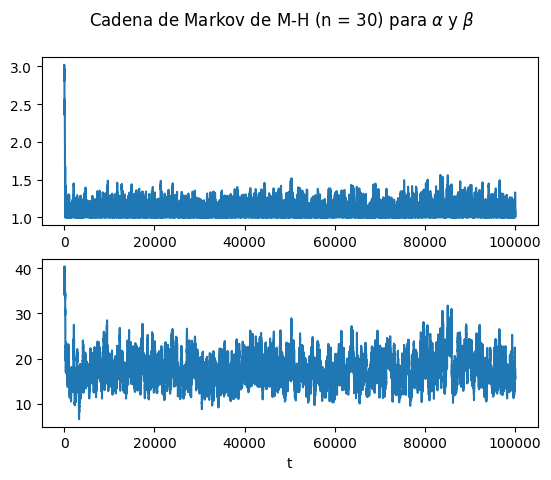
\includegraphics[width = 12 cm]{Figures/cadenaMarkov2.png} 
    \caption{Cadena de Markov de Metropolis-Hastings}
    \label{Fig. 1.06}
\end{figure} 

Notemos que tenemos una especie de convergencia hacia dentro de las curvas de nivel, es decir, se aproxima a simulaciones de la distribución objetivo. Para poder hablar de que la cadena producida es en efecto una muestra de la distribución objetivo, es necesario eliminar las primeras observaciones atípicas. Esto es llamado burn-in y para proceder calculamos el logaritmo de la densidad objetivo en cada punto de la cadena. Podemos ver en las siguientes figuras que tiende a estabilizarse
\begin{figure}[H] 
    \centering 
    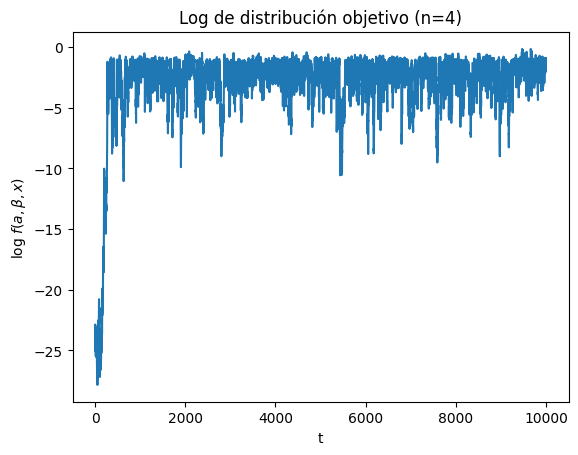
\includegraphics[width = 12 cm]{Figures/burn1.png} 
    \caption{Grafica del logaritmo de la densidad objetivo evaluado en cada punto de la cadena de Markov}
    \label{Fig. 1.07}
\end{figure} 
\begin{figure}[H] 
  \centering 
  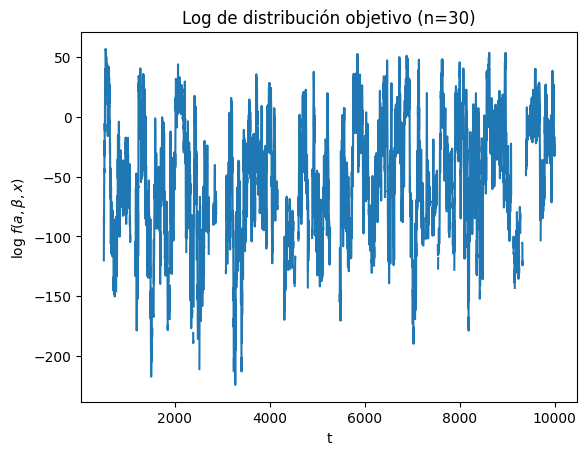
\includegraphics[width = 12 cm]{Figures/burn2.png} 
  \caption{Grafica del logaritmo de la densidad objetivo evaluado en cada punto de la cadena de Markov}
  \label{Fig. 1.08}
\end{figure} 
Para seleccionar el Burn-in notamos que para $n =4$ tenemos varios valles, entre ellos y más notable es el del extremos izquierdo, y un valle más pequeño pero notable por los 5000. Por tanto, elegimos un burn-in de 6000.

Posterior a remover las primeras 6000 iteraciones, hacemos un histograma de los valores observados para las marginales de $\alpha$ y $\beta$.
\begin{figure}[H] 
    \centering 
    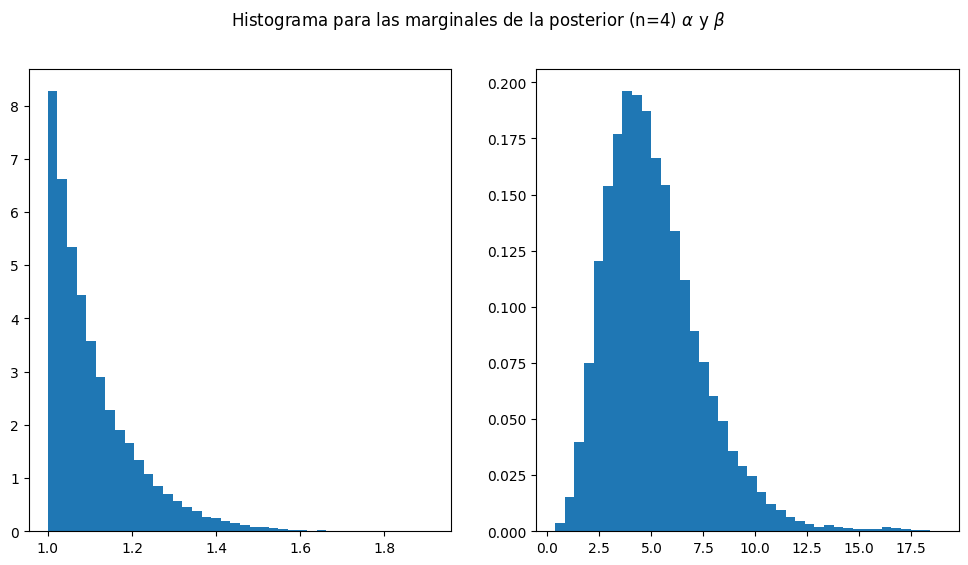
\includegraphics[width = 12 cm]{Figures/Histo1.png} 
    \caption{Histograma para $\alpha$ y $\beta$ en n = 4 de M-H }
    \label{Fig. 1.09}
\end{figure} 
\begin{figure}[H] 
  \centering 
  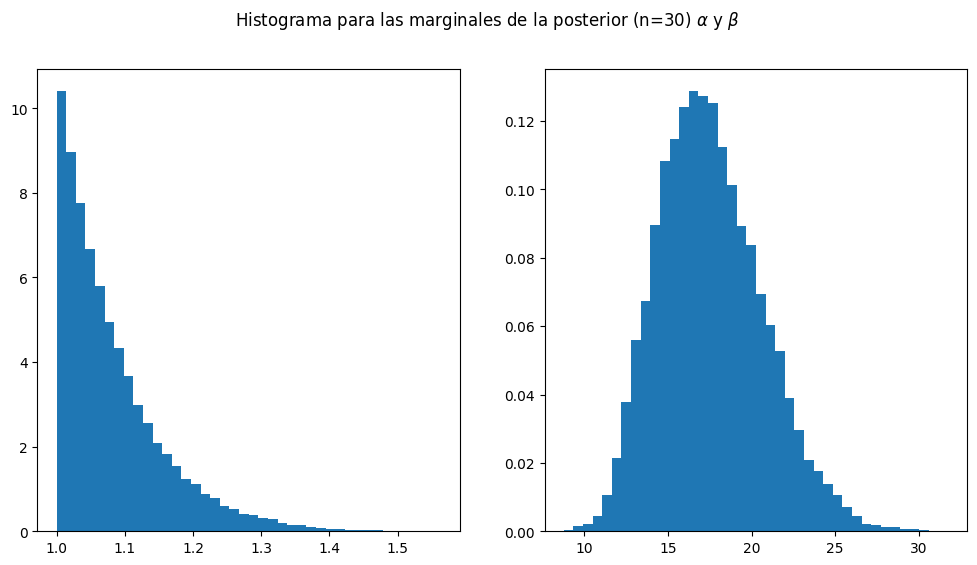
\includegraphics[width = 12 cm]{Figures/Histo2.png} 
  \caption{Histograma para $\alpha$ y $\beta$ en n = 30 de M-H }
  \label{Fig. 1.10}
\end{figure} 

Por último, consideramos otra distribución propuesta. Seleccionamos ahora un rectángulo uniforme. Es decir, sea $e_1 \sim U(-\varepsilon_1,\varepsilon)$ y $e_2 \sim U(-\varepsilon_2,\varepsilon_2)$ de forma que tomamos 
\begin{align*}
  \binom{\alpha_p}{\beta_p }  = \binom{\alpha}{\beta} + \binom{e_1}{e_2} 
\end{align*}

Para este análisis nos restringimos a revisar la trayectoria dada por el método Metropolis-Hastings que se muestra en las figuras siguientes
\begin{figure}[H] 
    \centering 
    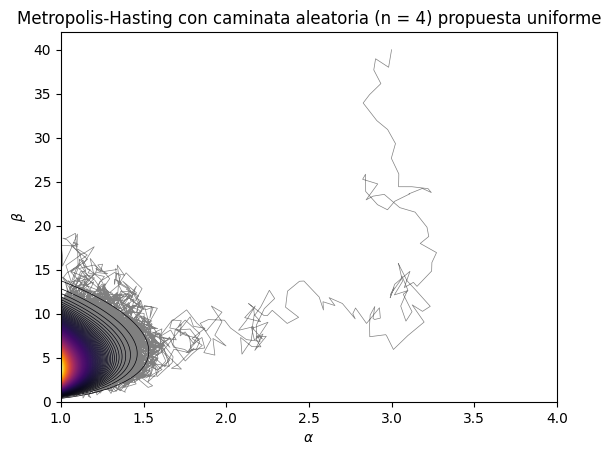
\includegraphics[width = 12 cm]{Figures/MHRWprop1.png} 
    \caption{Metropolis-Hastings con caminata aleatoria para la distribución objetivo con $n=4$}
    \label{Fig. 1.11}
\end{figure} 
\begin{figure}[H] 
    \centering 
    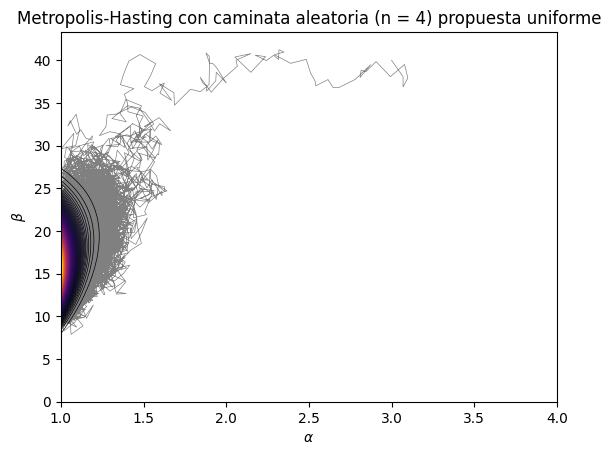
\includegraphics[width = 12 cm]{Figures/MHRWprop2.png} 
    \caption{Metropolis-Hastings con caminata aleatoria para la distribución objetivo con $n=4$}
    \label{Fig. 1.12}
\end{figure} 

Luego, la grafica para la evolución de la cadena de Markov es 
\begin{figure}[H] 
    \centering 
    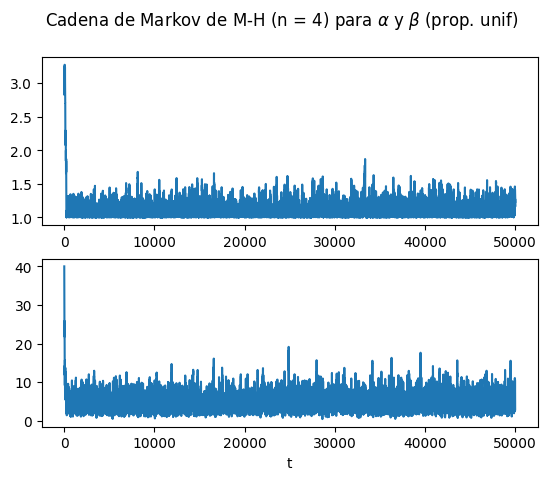
\includegraphics[width = 12 cm]{Figures/cadenaMarkov1Prop.png} 
    \caption{Cadena de Markov de Metropolis-Hastings para $n =4$}
    \label{Fig. 1.13}
\end{figure} 
\begin{figure}[H] 
    \centering 
    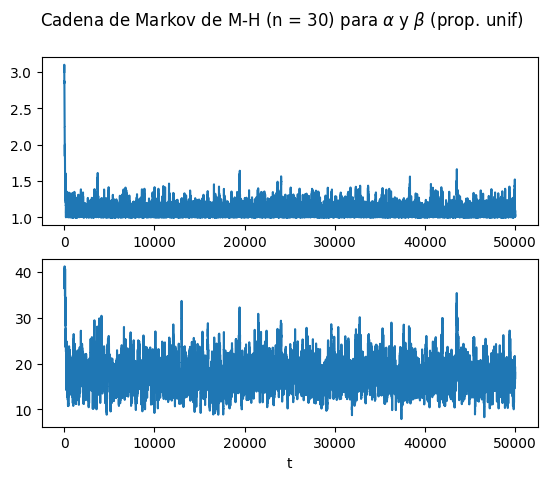
\includegraphics[width = 12 cm]{Figures/cadenaMarkov2Prop.png} 
    \caption{Cadena de Markov de Metropolis-Hastings para $n =30$}
    \label{Fig. 1.14}
\end{figure} 

Nuevamente tomaremos un burn-in de 6000. Tras la eliminación inicial mencionada, mostramos la evolución de la cadena para los próximos 200 paso. Vemos que está tiene varios rechazos ahí donde la grafica es constante, por lo que se puede pensar que tarda más en converger que con la propuesta normal.

\begin{figure}[H] 
    \centering 
    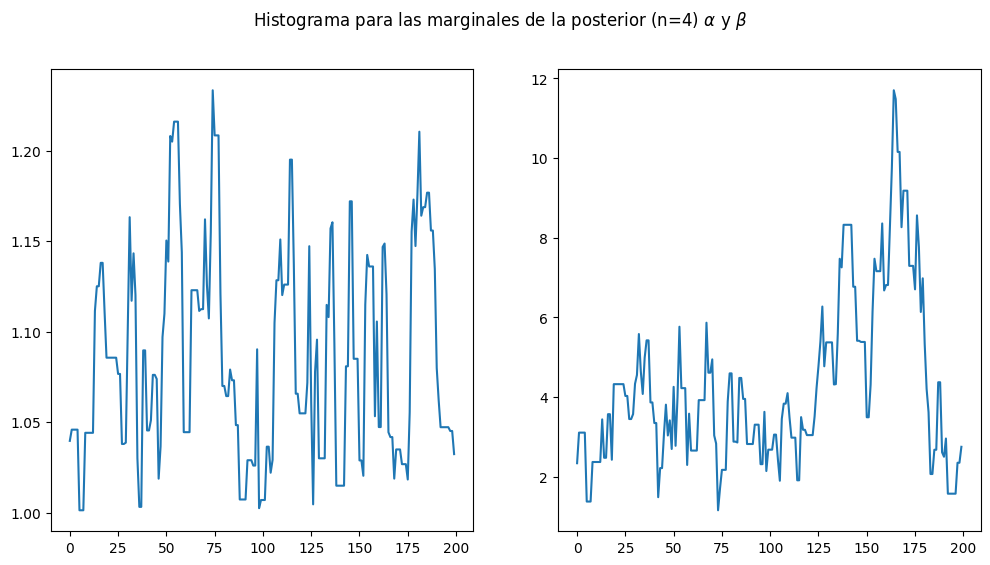
\includegraphics[width = 12 cm]{Figures/samplingprop1.png} 
    \caption{200 pasos para la cadena de Markov de Metropolis-Hastings con burn-in ya realizado.}
    \label{Fig. 1.15}
\end{figure} 
\begin{figure}[H] 
  \centering 
  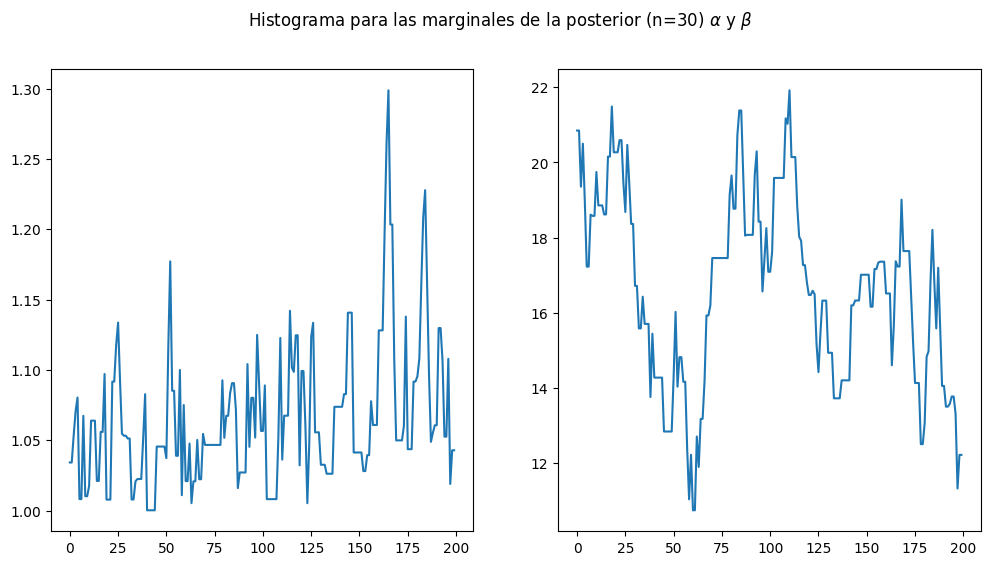
\includegraphics[width = 12 cm]{Figures/samplingprop2.png} 
  \caption{200 pasos para la cadena de Markov de Metropolis-Hastings con burn-in ya realizado.}
  \label{Fig. 1.16}
\end{figure} 


\end{solution}

\begin{problem}{2} 
  Simular de la distribución Gamma($\alpha$,1) con la propuesta Gamma($[\alpha], 1 $), donde $[a]$ denota la parte entera de $[a]$.

  Además, realizar el siguiente experimento: poner como punto inicial $x_0 = 900$ y graficar la evolución de la cadena, es decir, $f(X_t)$ vs $t$.
\end{problem}

\begin{solution} 
  

Para este inciso implementamos Metropolis-Hastings para simular de la distribución $Gamma(a,1)$ donde $a = $ 7.73 donde consideraremos primeramente la distribución propuesta $Gamma(\left [ a \right ],1)$ y $\left [ \cdot \right ]$ es la función parte entera.

Observemos que tenemos una propuesta independiente. Es decir, $q(y|x ) = q(y)$. Luego, la cadena de Markov cambiará de estado al propuesto con probabilidad $\rho$ de la forma
\begin{align}
  \rho(x,y ) &= \min\left \{ 1,\frac{f(y)}{f(x)}\frac{q(x|y)}{q(y|x)} \right \}\\
  &= \min\left \{ 1, \frac{\frac{1}{\Gamma(a)}y^{\alpha-1}e^{-y}}{\frac{1}{\Gamma(a)}x^{\alpha-1}e^{-x}} \cdot \frac{\frac{1}{\Gamma([a])}x^{[\alpha]-1}e^{-x}}{\frac{1}{\Gamma([a])}y^{[\alpha]-1}e^{-y}}\right \} \\
  &= \min \left \{ 1, \left ( \frac{y}{x} \right )^{\alpha - [\alpha]} \right \}
  \label{2.1}
\end{align}

Así, simulamos de la $Gamma(7,1)$ y hacemos M-H con el punto inicial $x_0 = 900$. Notemos de (\ref{2.1}) si $x$ es muy grande, entonces el cociente es pequeño y por tanto la probabilidad de aceptar la propuesta $y$ es muy baja. Luego, esperamos que en los primeros pasos tengamos que el estado de la cadena no cambia, es decir se mantiene en 900. Por tanto, es necesario hacer un burn-in para poder usar los datos como simulación de la distribución objetivo. Veamos la cadena en las 30000 iteraciones calculadas

\begin{figure}[H] 
    \centering 
    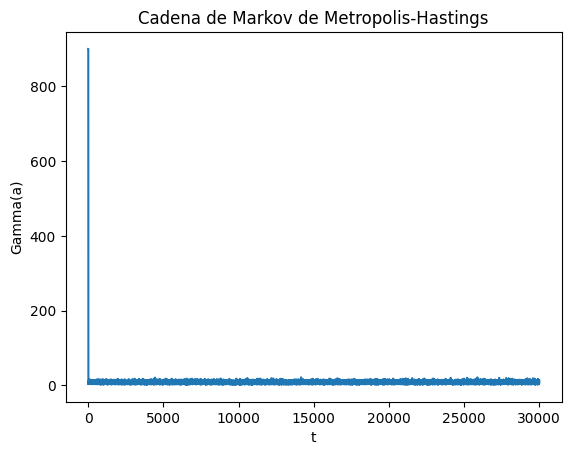
\includegraphics[width = 14 cm ]{Figures/2_cadena.png} 
    \caption{Cadena de Markov para M-H con distribución objetivo Gamma(a,1)}
    \label{Fig. 2.01 }
\end{figure} 

Para tener más claro la cantidad de Burn-in grafiquemos la cadena para los primeros 50 pasos
\begin{figure}[H] 
    \centering 
    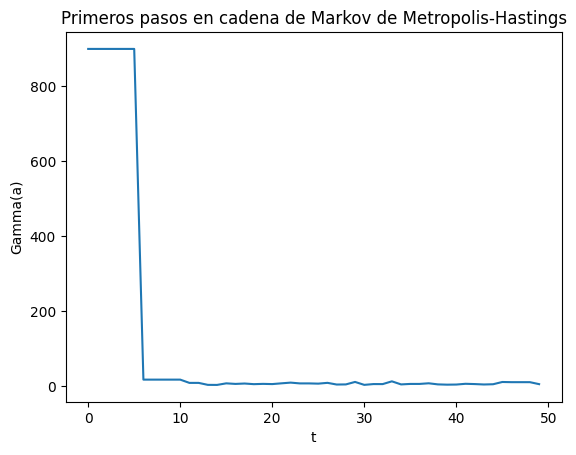
\includegraphics[width = 14 cm ]{Figures/2_cadenaInicio.png} 
    \caption{Cadena de Markov para M-H en los primeros 50 pasos.}
    \label{Fig. 2.02}
\end{figure} 
Dependiendo la semilla o la realización, la cantidad de veces que se rechaza la propuesta manteniendo la posición inicial puede variar. En nuestro caso tenemos que dicho cambio está un poco antes del paso 10. Sin embargo, haciendo experimentos se pudo encontrar casos que superaban los 50 pasos. Por lo pronto y para este caso, tomamos un burn-in de 50.

De la cadena de Markov, ya aplicado el burn-in podemos obtener un histograma y comparar con la densidad objetivo
\begin{figure}[H] 
    \centering 
    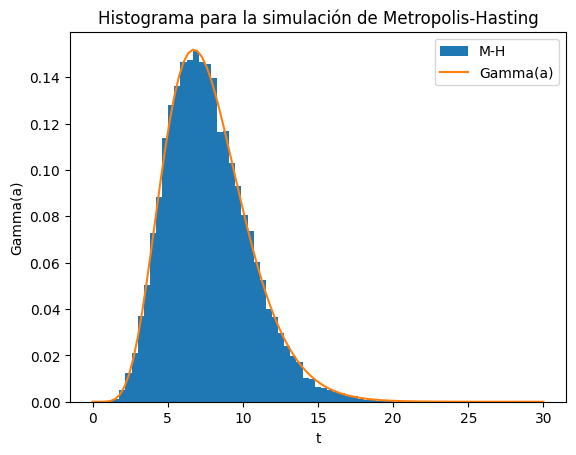
\includegraphics[width = 14 cm ]{Figures/2_histo.png} 
    \caption{Histograma de la simulación obtenida por el método de Metropolis-Hastings}
    \label{Fig. 2.03}
\end{figure}  

La cadena es bastante óptima, se aproxima bastante rápido a la distribución objetivo, lo cual tiene sentido ya que existe cierta continuidad en los parámetros de la distribución gamma y estos se encuentra cercanos, pues la distancia para el parámetro $\alpha$ no supera uno.

Se propone ahora usar la distribución propuesta como la uniforme en [0,30] ya que el soporte para la gamma está concentrado en este intervalo. Luego, por el método M-H tenemos que eliminar el burn-in, que para este caso y por construcción se puede permitir ser más bajo ya que el punto inicial bajará con alta probabilidad. Como podemos ver en las gráficas para la cadena de Markov

\begin{figure}[H] 
    \centering 
    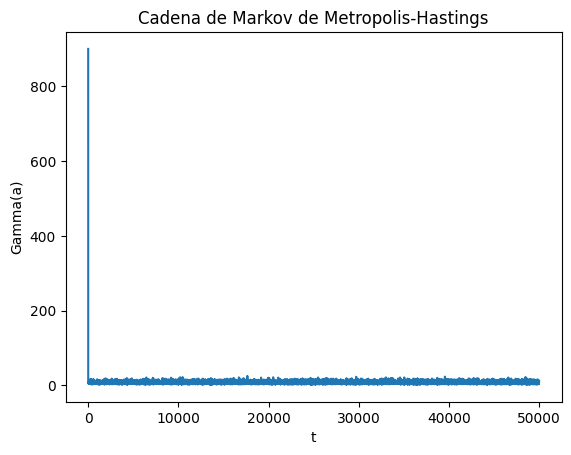
\includegraphics[width = 14 cm ]{Figures/2_unif.png} 
    \caption{Cadena de Markov para la propuesta uniforme}
    \label{Fig. 2.04}
\end{figure} 

\begin{figure}[H] 
    \centering 
    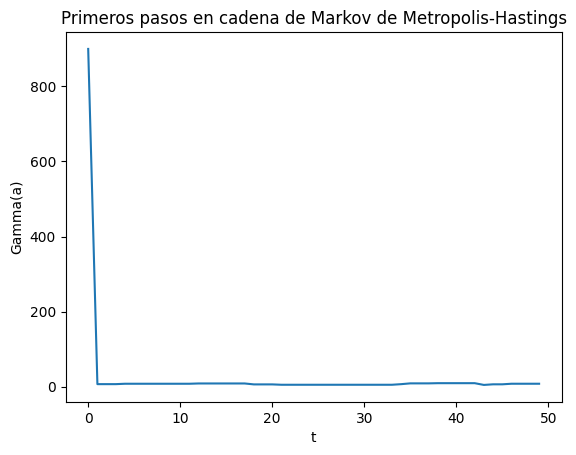
\includegraphics[width = 14 cm ]{Figures/2_unif_inicio.png} 
    \caption{Primeros valores de la cadena de Markov para M-H con propuesta uniforme}
    \label{Fig. 2.05}
\end{figure} 

Por último, eliminando el burn-in y tomando el histograma con la simulación es
\begin{figure}[H] 
    \centering 
    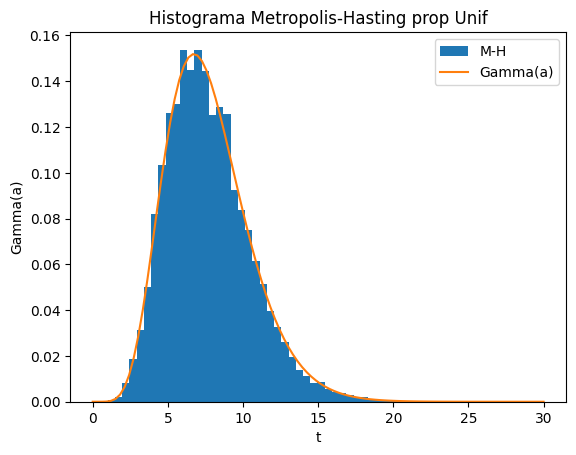
\includegraphics[width = 14 cm]{Figures/2_histo_unif.png} 
    \caption{Histograma para simulación M-H con propuesta uniforme.}
    \label{Fig. 2.06}
\end{figure} 


\end{solution}

\begin{problem}{3} 
  Implementar Random Walk Metropolis Hasting (RWMH) donde la distribución objetivo es $\mathcal{N}_2 \left( \mu, \Sigma  \right)$, con 
  \begin{align*}
    \mu = \binom{3}{5} \:\:\:\:\: \Sigma = \begin{pmatrix}
      1 & 0.9 \\ 
      0.9 & 1 
      \end{pmatrix}.
  \end{align*}
  Utilizar como propuesta $\varepsilon_i \sim \mathcal{N}_2(0,\sigma^2I)$ ?` Cómo elegir $\sigma$ para que la cadena sea eficiente ? ?` Qué consecuencias tiene la elección de $\sigma$ ?

  Como experimento, elige como punto inicial $x_0 = \binom{1000}{1}$ y comenta los resultados.
\end{problem}

% \textbf{Para todos los incisos del ejercicio anterior:}
% \begin{enumerate}
%   \item Establece cual es tu distribución inicial .
%   \item Grafica la evolución de la cadena.
%   \item Indica cuál es el Burn-in.
%   \item Comenta qué tan eficiente es la cadena.
%   \item Implementa el algoritmo MH considerando una propuesta diferente.
% \end{enumerate}

\begin{solution} 
  
\end{solution}

\begin{thebibliography}{9}

    \bibitem{Casella}
    Robert, C. P., Casella, G., and Casella, G. (1999). Monte Carlo statistical methods (Vol. 2). New York: Springer.

    \bibitem{Wasserman}
    Wasserman, L. (2004). All of statistics: a concise course in statistical inference (p. 413). New York: Springer.
    
\end{thebibliography}
      




    \end{document}